\section{Multiple Linear Regression}

Model Formula and assumptions: $Y_i = \sum_{j=1}^p \beta_j x_{ij} + \epsilon_i \ \Leftrightarrow \ Y = X \beta + \epsilon \ \Leftrightarrow \ Y_i = x_i^T \beta + \epsilon_i \ \Leftrightarrow \ Y_i = \beta_1 + \sum_{j=2}^p X_{ij} \beta_j + \epsilon_i$ where $\epsilon_1,\dots,\epsilon_n \stackrel{\text{iid}}{\sim} \mathcal{N}(0,\sigma^2)$ hence $\Cov(\epsilon) = \sigma^2 \id$. Assume $n \geq p$ and thus $X$ has full rank.

\vspace{4pt}

\fat{Least Squares Model}
$\hat{\beta} = \argmin \Norm{Y - X \beta}_2^2 = (X^T X)^{-1} X^T Y$. Def: $\epsilon_i \approx Y_i - x_i^T \beta := r_i \ \Rightarrow \ \hat{\sigma}^2 = \frac{1}{n-p} \sum_{i=1}^n r_i^2$.

\vspace{4pt}

\fat{Assumptions:} 1) LinRegEq is correct ($\Expec \eckigeklammer{\epsilon_i} = 0$), 2) $x_i$'s are exact, 3) Var of Errors is const ($\Var(\epsilon_i) = \sigma^2$) ("Homoscedasticity"), 4) Errors are uncorrelated ($\Cov(\epsilon_i,\epsilon_j) = 0$), 5) Errors $\epsilon_i$ are jointly normally distributed $\Rightarrow$ $Y_i$'s are jointly normally distributed.

\vspace{4pt}

\fat{Geometric Interpretation}
$X \hat{\beta}$ is the orthogonal projection of $Y$ onto $\mathcal{X} \equiv$ span$(X)$ (columnwise span) $\Rightarrow \ \hat{Y} = X \hat{\beta} = \underbrace{X (X^T X)^{-1} X^T}_{:= P} Y$. $\mathcal{X}$ is a $p$-dim subspace of $\R^n$, $P = P^T = P^2$, $\tr(P) = \tr(\id_p) = p$. The residuals live in $\mathcal{X}^\perp$: $\vec{r} = (1-P) \vec{Y}$.

%\paragraph{Estimating $\beta_j$'s:} $H_{0,j}: \ \beta_j = 0$, std.error: $\sqrt{\widehat{\Var}(\hat{\beta}_j)}$

\vspace{-5pt}

\subsection{Properties of LS Estimator}
(i) $\Expec\eckigeklammer{\hat{\beta}} = \beta$ hence $\hat{\beta}$ is an unbiased estimator,
(ii) $\Expec\eckigeklammer{\hat{Y}} = \Expec\eckigeklammer{Y} = X \beta$, $\Expec\eckigeklammer{r} =0$,
(iii) $\Cov(\hat{\beta}) = \sigma^2 \klammer{X^T X}^{-1}$,
(iv) $\Cov(\hat{Y}) = \sigma^2 P$, $\Cov(r) = \sigma^2 (1-P)$,
(v) $\Var(r_i) = \sigma^2 (1-P_{ii})$ hence $\Expec\eckigeklammer{\sum_i r_i^2} = \sum_i \Var(r_i) = \sigma^2 (n-\tr(P)) = \sigma^2 (n-p)$ hence $\Expec\eckigeklammer{\hat{\sigma}} = \Expec\eckigeklammer{\frac{1}{n-p} \sum_i r_i^2} = \sigma$ hence an unbiased estimator,
(vi) $\hat{\beta} \sim \mathcal{N}_p \klammer{\beta,\sigma^2 \klammer{X^T X}^{-1}}$, $\hat{Y} \sim \mathcal{N}_n \klammer{X \beta,\sigma^2 P}$, $r \sim \mathcal{N}_n \klammer{0,\sigma^2 (1-P)}$, $\hat{\sigma}^2 \sim \frac{\sigma^2}{n-p} \chi_{n-p}^2$

\vspace{-5pt}

\subsection{Tests and Confidence Regions}
$H_{0,j}: \ \beta_j = 0$, std.error: $\sqrt{\widehat{\Var}(\hat{\beta}_j)}$. Thus: $\frac{\hat{\beta}_j}{\sqrt{\sigma^2 (X^T X)_{jj}^{-1}}} \sim \mathcal{N}(0,1)$ under $H_{0,j}$ and $T_j = \frac{\hat{\beta}_j}{\sqrt{\hat{\sigma}^2 \klammer{X^T X}_{jj}^{-1}}} \sim t_{n-p}$ under $H_{0,j}$. Conf Int: $\hat{\beta}_j \pm \sqrt{\hat{\sigma}^2 \klammer{X^T X}_{jj}^{-1}} \cdot t_{n-p;1-\frac{\alpha}{2}}$

\vspace{4pt}

\fat{Test of global $H_0$}
$H_0$: $\beta_2 = \dots = \beta_p = 0$, $H_A$: $\exists j \in \geschwungeneklammer{2,\dots,p}: \beta_j \neq 0$.
$F = \frac{\Norm{\hat{Y} - \bar{Y}}_2^2 / (p-1)}{\Norm{Y - \hat{Y}}_2^2 / (n-p)} \sim F_{p-1,n-p}$ under $H_0$.
$R^2 = \frac{\Norm{\hat{Y} - \bar{Y}}_2^2}{\Norm{Y - \hat{Y}}_2^2} = 1 - \frac{\Norm{Y - \hat{Y}}_2^2}{\Norm{Y-\bar{Y}}_2^2}$

\vspace{4pt}

\fat{Confidence Lvls} We say a Test $T_n : \mathcal{X}^n \rightarrow \geschwungeneklammer{0,1}$ is (i) lvl $\alpha$ if: $\sup_{P \in H_0} \mathbb{P}_{P^n} (T_n = 1) \leq \alpha$, (ii) pointwise asymptotic lvl $\alpha$ if $\sup_{P \in H_0} \lim_{n \rightarrow \infty} \mathbb{P}_{P^n} (T_n = 1) \leq \alpha$, (iii) uniform asymptotic lvl $\alpha$ if $\lim_{n \rightarrow \infty} \sup_{P \in H_0} \mathbb{P}_{P^n} (T_n = 1) \leq \alpha$

\vspace{4pt}

\fat{p-value} Infimum over all significance lvl's $\alpha$ s.t. test rejects.

\vspace{4pt}

\fat{For new $x_0$:}
Confidence Interval: $\frac{x_0^T \hat{\beta} - x_0^T \beta}{\hat{\sigma} \sqrt{x_0^T \klammer{X^T X}^{-1} x_0}} \sim t_{n-p}$,

Prediction Interval: $\frac{y_0 - x_0^T \hat{\beta}}{\hat{\sigma} \sqrt{1 + x_0^T \klammer{X^T X}^{-1} x_0}} \sim t_{n-p}$

\vspace{-5pt}

\subsection{Analysis of Residuals \& Checking of Model Assumptions}

\vspace{-5pt}

\paragraph{Tukey-Anscombe Plot} Plot $r_i$ vs. $\hat{Y}_i$'s.

\vspace{2pt}

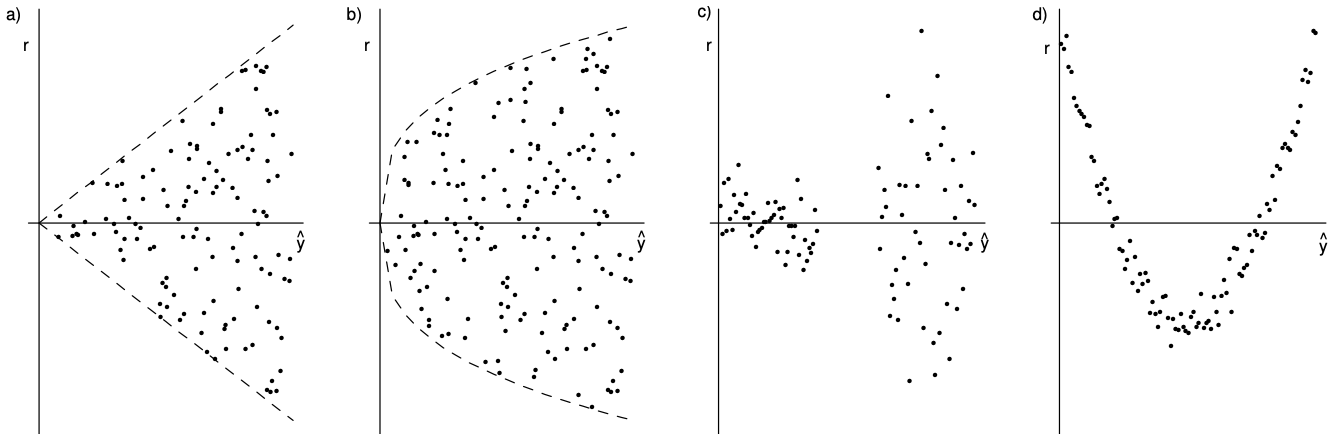
\includegraphics[width=0.49\textwidth]{Bilder/TukeyAnscombe.png}

\vspace{1pt}

a) Linear increase of sd (solution: log-transform), b) non-linear increase of sd, c) 2 groups with different variances, d) missing quadratic term in the model

\vspace{-5pt}

\paragraph{QQ-Plot} Plot empirical quantiles vs. theoretical quantiles of $\mathcal{N}(0,1)$. If $r \sim \mathcal{N}(\mu,\sigma^2)$, then plot would be a straight line.

\vspace{1pt}

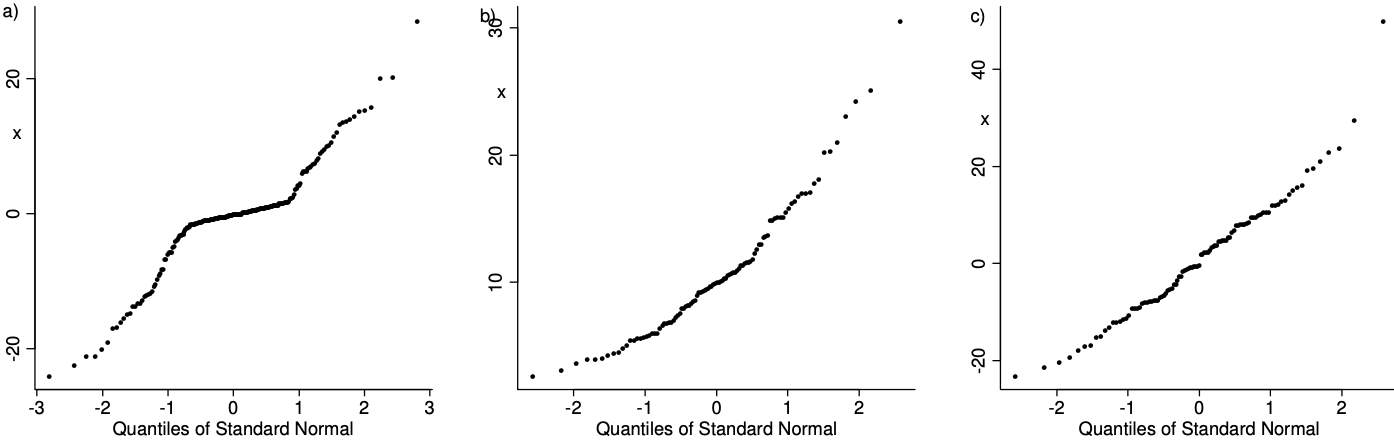
\includegraphics[width=0.4\textwidth]{Bilder/QQPlot.png}

\vspace{1pt}

a) long-tailed distribution, b) skewed distribution, c) dataset with outlier

\subsection{Generalized LS and weighted Regression}
$Y = X \beta + \epsilon$, $\epsilon \sim \mathcal{N}_n(0,\SigmaCov)$, $\SigmaCov$ known and $\SigmaCov = C C^T$. Reformulate: $\tilde{Y} = \tilde{X} \beta + \tilde{\epsilon}$ with $\tilde{Y} = C^{-1} Y$, $\tilde{X} = C^{-1} X$, $\tilde{\epsilon} \sim \mathcal{N}_n (0,\id)$ and obtain: $\hat{\beta} = \klammer{X^T \SigmaCov^{-1} X}^{-1} X^T \SigmaCov^{-1} Y$, $\Cov(\hat{\beta}) = \klammer{X^T \SigmaCov^{-1} X}^{-1}$

\vspace{1pt}

Special Case: $\SigmaCov = \sigma^2 \text{diag}(z_1,\dots,z_n)$ $\Rightarrow$ weighted LS problem: $\min_\beta \sum_{i=1}^n w_i \klammer{Y_i - x_i^T \beta}$, $w_i = \frac{1}{z_i}$

\vspace{-5pt}

\subsection{Model Selection}
Maybe some $\beta_j$'s are irrelevant. If $p>n$, $X^T X$ is not invertible anymore and $\hat{\beta} \argmin_\beta \Norm{Y - X \beta}_2^2$ not unique anymore and $\Expec\eckigeklammer{X \hat{\beta}} \neq X \beta$. Approach: $Y_i \approx \sum_{r=1}^q \hat{\beta}_{j_r} x_{i,j_r} =: \hat{m}_{\geschwungeneklammer{j_1,\dots,j_q}} (\vec{x}_i)$, $j_l \in \geschwungeneklammer{1,\dots,p}$. $aMSE = \frac{1}{n} \sum_{i=1}^{n} \Expec \eckigeklammer{\klammer{m(\vec{x}_i) - \hat{m}_q (\vec{x}_i)}^2} = \frac{1}{n} \sum_{i=1}^{n} \klammer{\Expec \eckigeklammer{\hat{m}_q (\vec{x}_i)} - m(\vec{x}_i)}^2 + \frac{1}{n} \sum_{i=1}^{n} \Var(\hat{m}_q (\vec{x}_i)) = \frac{1}{n} \sum_{i=1}^{n} \klammer{\Expec \eckigeklammer{\hat{m}_q (\vec{x}_i)} - m(\vec{x}_i)}^2 + \frac{q}{n} \sigma^2$

\vspace{4pt}

\fat{Penelized Regression (Mellows $C_p$ Statistic)}
$\hat{\beta}_\lambda = \argmin_\beta \Norm{Y - X \beta}_2^2 + \lambda \Norm{\beta}_0$. $\lambda$ large $\rightarrow$ fewer variables. $C_p = \frac{\Norm{Y - X_\mathcal{M} \hat{\beta}_{\mathcal{M}}}_2^2}{\sigma_{\mathcal{M}}^2} - n + 2 (n-df_{residuals})$. Akaike's Information Criterion (AIC) $\Leftrightarrow$ Mellows $C_p$ for Gaussian Models: $\lambda = 2 \hat{\sigma}^2$. Bayese Information Criterion (BIC): $\lambda = \log(n) \hat{\sigma}^2$

\vspace{4pt}

\fat{Searching for best Model}
\underline{Forward Selection:} Start with smallest model and iteratively add a predictor variable that reduces RSS the most. You obtain a seq of Models $\mathcal{M}_0 \subseteq \mathcal{M}_1 \subseteq \dots$. Chose $\mathcal{M}_i$ that minimizes $RSS_\lambda$. \underline{Backward Selection:} Start with full model and iteratively exclude pred. vars that increase RSS the least ($\mathcal{M}_0 \supseteq \mathcal{M}_1 \supseteq ...$) and chose $\mathcal{M}_i$ that minimizes $RSS_\lambda$.
